\documentclass[border=10pt]{standalone}
\usepackage[svgnames]{xcolor}
\usepackage{amsmath}
\usepackage{pgfplots}
\pgfplotsset{compat=newest}
\usepackage[sfdefault]{FiraSans}
\usepackage{FiraMono}
\renewcommand*\familydefault{\sfdefault}
\begin{document}
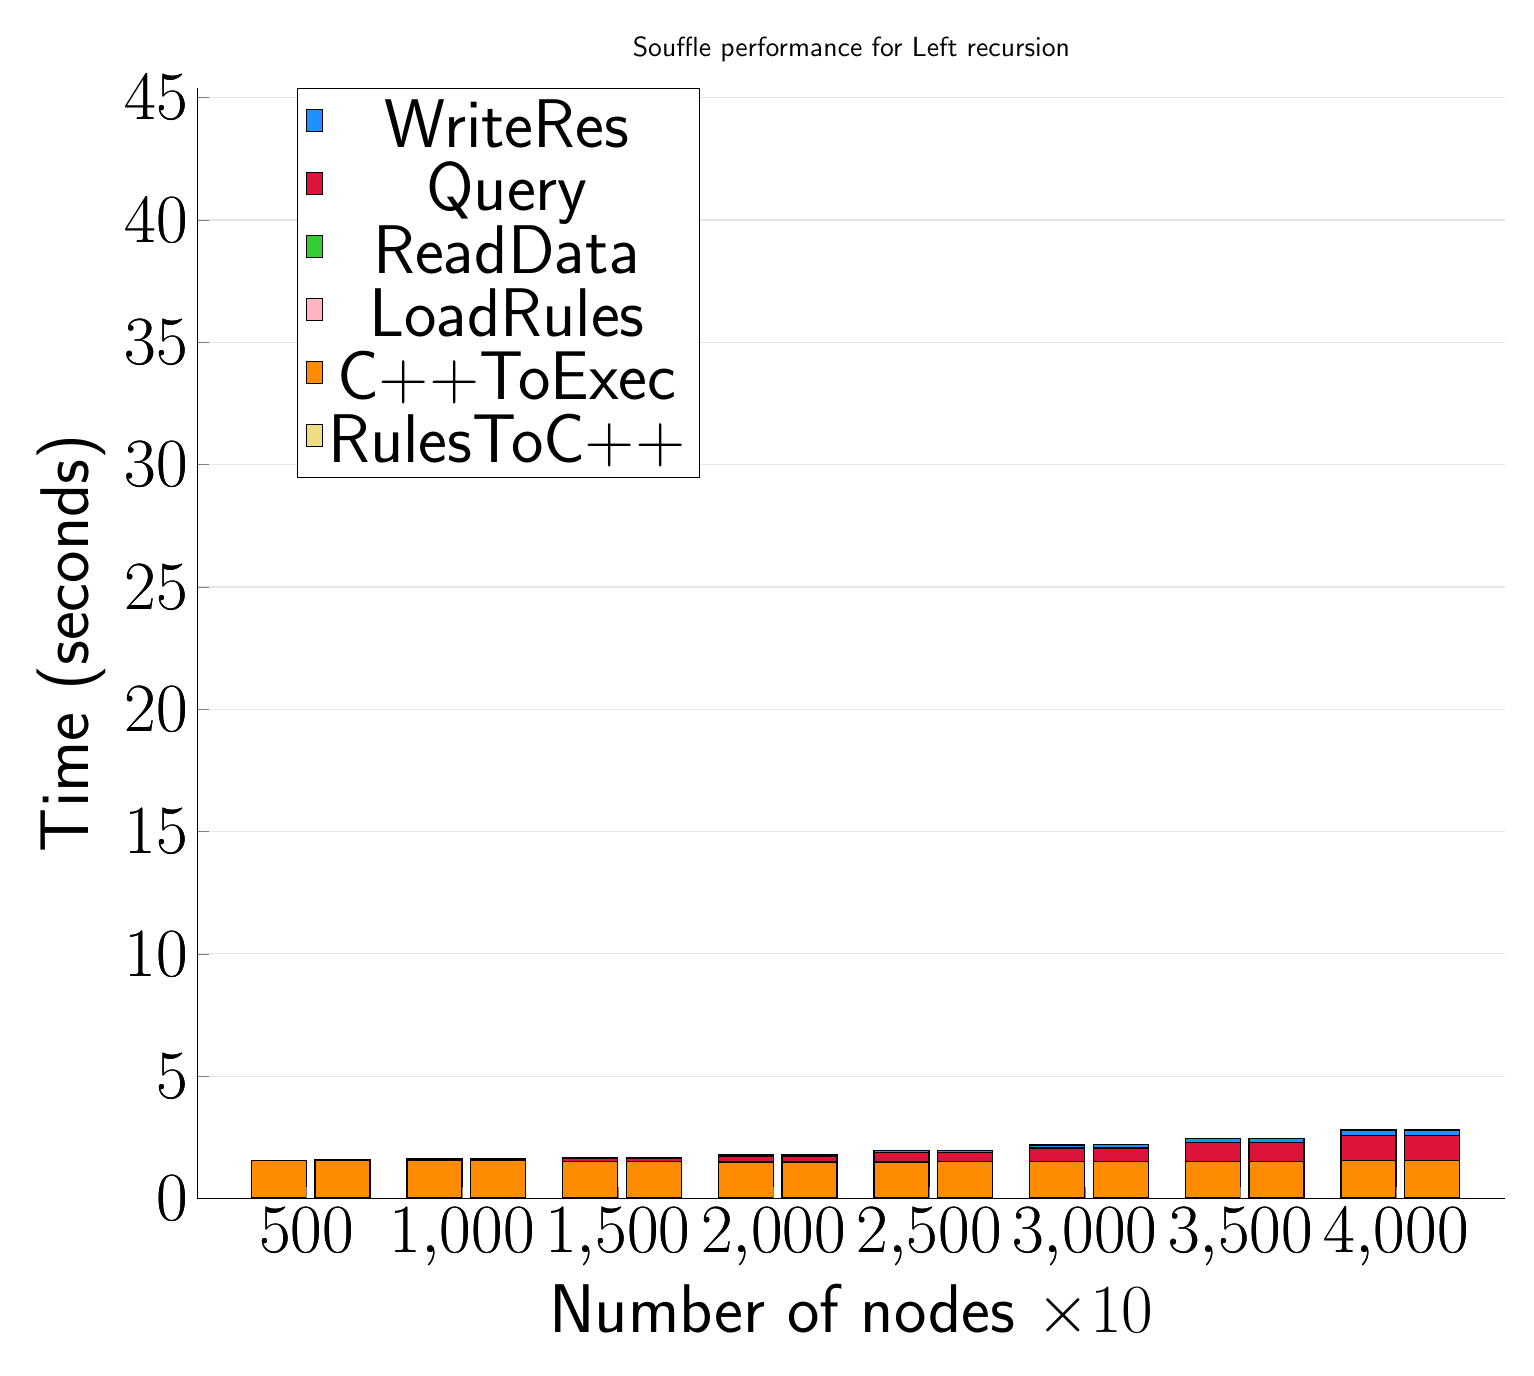
\begin{tikzpicture}
\begin{axis}[
   ybar stacked,
   title={Souffle performance for Left recursion},
   bar shift=-10pt,
   width=1.5\textwidth,
   bar width=0.7cm,
   ymajorgrids, tick align=inside,
   major grid style={draw=gray!20},
   xtick=data,
   ymin=0, ymax=45.40037,
   axis x line*=bottom,
   axis y line*=left,
   enlarge x limits=0.1,
   legend style={
       at={(0.23, 1)},
       anchor=north,
       legend columns=1,
       font=\Huge,
   },
   ylabel={Time (seconds)},
   xlabel={Number of nodes $\times 10$},
   label style={font=\Huge},
   tick label style={font=\Huge},
]
\addlegendimage{fill=DodgerBlue, draw=black, line width=0.2pt}
\addlegendentry{WriteRes}
\addlegendimage{fill=Crimson, draw=black, line width=0.2pt}
\addlegendentry{Query}
\addlegendimage{fill=LimeGreen, draw=black, line width=0.2pt}
\addlegendentry{ReadData}
\addlegendimage{fill=LightPink, draw=black, line width=0.2pt}
\addlegendentry{LoadRules}
\addlegendimage{fill=DarkOrange, draw=black, line width=0.2pt}
\addlegendentry{C++ToExec}
\addlegendimage{fill=LightGoldenrod, draw=black, line width=0.2pt}
\addlegendentry{RulesToC++}
\addplot +[fill=LightGoldenrod, draw=black, line width=0.5pt] coordinates {
    (500, 0.040999984741210936)
    (1000, 0.04100000858306885)
    (1500, 0.039999985694885255)
    (2000, 0.04100003242492676)
    (2500, 0.040999984741210936)
    (3000, 0.03900003433227539)
    (3500, 0.040999984741210936)
    (4000, 0.039999961853027344)
};
\addplot +[fill=DarkOrange, draw=black, line width=0.5pt] coordinates {
    (500, 1.5050000429153443)
    (1000, 1.522000002861023)
    (1500, 1.4650000095367433)
    (2000, 1.446999979019165)
    (2500, 1.4509999990463256)
    (3000, 1.4639999628067017)
    (3500, 1.4700000047683717)
    (4000, 1.509000015258789)
};
\addplot +[fill=LightPink, draw=black, line width=0.5pt] coordinates {
    (500, 8.26458e-05)
    (1000, 7.491690000000001e-05)
    (1500, 0.00010965819999999999)
    (2000, 0.00010886669999999999)
    (2500, 0.00011241259999999998)
    (3000, 0.0001003959)
    (3500, 9.672089999999999e-05)
    (4000, 0.00010314179999999998)
};
\addplot +[fill=LimeGreen, draw=black, line width=0.5pt] coordinates {
    (500, 0.0011102714)
    (1000, 0.001919933)
    (1500, 0.0035170970000000003)
    (2000, 0.0044951539999999995)
    (2500, 0.005504755)
    (3000, 0.006572262000000001)
    (3500, 0.0070333470000000006)
    (4000, 0.008018342000000001)
};
\addplot +[fill=Crimson, draw=black, line width=0.5pt] coordinates {
    (500, 0.0149091)
    (1000, 0.05864585)
    (1500, 0.1352838)
    (2000, 0.23860159999999997)
    (2500, 0.37622380000000005)
    (3000, 0.5550203)
    (3500, 0.7665172)
    (4000, 1.020129)
};
\addplot +[fill=DodgerBlue, draw=black, line width=0.5pt] coordinates {
    (500, 0.004382641)
    (1000, 0.01432533)
    (1500, 0.03193746000000001)
    (2000, 0.056822399999999995)
    (2500, 0.08855163)
    (3000, 0.1270181)
    (3500, 0.1737641)
    (4000, 0.2262083)
};
\end{axis}
\begin{axis}[
   ybar stacked,
   bar shift=13pt,
   width=1.5\textwidth,
   bar width=0.7cm,
   ymajorgrids, tick align=inside,
   major grid style={draw=none},
   xtick=data,
   ymin=0, ymax=45.40037,
   axis x line*=none,
   axis y line*=none,
   enlarge x limits=0.1,
   label style={font=\Huge},
   tick label style={font=\Huge},
]
\addplot +[fill=LightGoldenrod, draw=black, line width=0.5pt] coordinates {
    (500, 0.030000000000000006)
    (1000, 0.030000000000000006)
    (1500, 0.030000000000000006)
    (2000, 0.030000000000000006)
    (2500, 0.030000000000000006)
    (3000, 0.030000000000000006)
    (3500, 0.030000000000000006)
    (4000, 0.030000000000000006)
};
\addplot +[fill=DarkOrange, draw=black, line width=0.5pt] coordinates {
    (500, 1.522)
    (1000, 1.5400000000000003)
    (1500, 1.4850000000000003)
    (2000, 1.4700000000000002)
    (2500, 1.473)
    (3000, 1.483)
    (3500, 1.4889999999999999)
    (4000, 1.525)
};
\addplot +[fill=LightPink, draw=black, line width=0.5pt] coordinates {
    (500, 8.209999999999999e-05)
    (1000, 7.439999999999999e-05)
    (1500, 0.00010890000000000002)
    (2000, 0.00010740000000000001)
    (2500, 0.00011150000000000001)
    (3000, 9.92e-05)
    (3500, 8.58e-05)
    (4000, 0.00010250000000000001)
};
\addplot +[fill=LimeGreen, draw=black, line width=0.5pt] coordinates {
    (500, 0.0011086)
    (1000, 0.0019181000000000003)
    (1500, 0.0035159999999999996)
    (2000, 0.004493200000000001)
    (2500, 0.005503900000000001)
    (3000, 0.006535400000000001)
    (3500, 0.007031999999999999)
    (4000, 0.0080124)
};
\addplot +[fill=Crimson, draw=black, line width=0.5pt] coordinates {
    (500, 0.0148894)
    (1000, 0.058338999999999995)
    (1500, 0.13507059999999999)
    (2000, 0.23820510000000006)
    (2500, 0.37549179999999993)
    (3000, 0.5541748)
    (3500, 0.7649524000000001)
    (4000, 1.018127)
};
\addplot +[fill=DodgerBlue, draw=black, line width=0.5pt] coordinates {
    (500, 0.004368199999999999)
    (1000, 0.014265799999999999)
    (1500, 0.031566500000000004)
    (2000, 0.0564145)
    (2500, 0.08798500000000001)
    (3000, 0.1261758)
    (3500, 0.17266189999999998)
    (4000, 0.22527880000000003)
};
\end{axis}
\end{tikzpicture}

\end{document}
